\documentclass[12pt]{article}
\usepackage[hmargin=2.0cm,vmargin=1cm]{geometry}
\usepackage[utf8]{inputenc}
\usepackage{graphicx}
\usepackage{float}
\usepackage{cite}
\usepackage{natbib}
\usepackage{amsmath}

\title{\begin{LARGE}
{Modelling the Sagittarius stream}
\end{LARGE}}
\begin{document}
\maketitle

Some characteristics

\begin{itemize}
\item First observed by Ibata 94
\item Large population of young relatively metal rich Sgr M-giant wrapping 360
across the sky  (Majewski 03)
\item debris streamer continues through the North Galactic Pole passes over the 
solar neighborhood toward the galactic anitcenter. (Belokurov 06)
\item Evolution in metallicity distribution function.
\end{itemize}

Efforts trying to modelled the stream.

\begin{itemize}
\item Johnston 95, 99
\item Velazquez \& White 95
\item Edlesohn \& Elmegreen 97
\item Ibata et al 07
\item Gomez-Flechoso et al 99
\item Helmi \& White 2001
\item Martinez-Delgado et al 2004
\end{itemize}

MW DM halo:

\begin{itemize}
\item Ibata et al 01 (Spherical)
\item Helmi 04 (Prolate)
\item Johnston et al 05 (Oblate halo)
\item Law et al 05
\item Fellhauer et al 06 (Spherical)
\item Martinez Delgado et al 07 (Oblate)
\item Law, Majewski, Johnston 09 ()
\item Law \& Majewski (Triaxial)
\end{itemize}

\section{The Milky Way Dark Matter halo}
\subsection{Vera Ciro13}

\citep{Vera13} study a dark matter halo that is oblate in the center
 and triaxial in the outskirts. 

This study is motivated by expectations that the disk would modify the 

The motivations are that the disk is expected
 to modify the

 inner halo shape towards one that is oblate, in which case disk stability 
is ensured.  

also if the
halo is oblate at the inner the disk stability is ensured. 

They
argue that the triaxial halo configuration of \citep{Law10} it's
not common in the LCDM model due to the small c/a ratio compared to
LCDM predictions.

*** Is this actually an issue - can’t the MW be an outlier?   
***  How much of an outlier is the Law model vs average properties


They integrate orbits of test particles in the potential Eq.\ref{eq:vera} for a period
of 2gyr backwards and forwards. 

For every test particle they select 10 random locations 
in its orbit and store the position and velocity. 
orbit of this test particle from which they have positions and velocities.

 With this methodology they reproduce observables that might be compared with 
the Sgr stream.

The results from this numerical experiment is that 

They find  a good fit in some
parts of the orbits (see Fig.2 of that paper) and that the fit does not depend
strongly on the parameter $r_a$ of the halo potential.

In the second part of this paper they study the effect of torques in the Sgr
stream. The authors argue that there are two torques, one from the triaxiality
of the halo itself and the other due to the LMC. Interestingly, the major
axis of the triaxial potential in \citep{Law10} is in the direction towards
 the LMC. They studied the magnitude of both torques and found that both
have an equal effect on the Sgr stream.

As a result, they modify the parameters of the halo model in order to account
for the additional torque of the LMC, these new parameters are now more consistent
 with those expected from the LCDM model. For the orbit integration they also take
into account the potential of the LMC. With these considerations, they find a better fit for  the Sgr
stream (see Fig.5 of that paper).

\section{How common is the Milky Way}

\subsection{There’s no place like home? Statistics of Milky Way-mass dark matter
haloes (MBK10)}

The MW dark matter halo range between [$1\times 10^{12} - 3\times 10^{12}$]
typical $Rvir = 200 h^{-1}$. It is not common to have large satellites as
the MW. 

\subsection{The shape of the gravitational potential in cold dark matter haloes (Hayashi07)}

Goal: Study the shape of the gravitational potential of CDM halos. Radial dependence of triaxilaity in the potential of CDM halos. 
Results: Near the center the halo is prolate $c/a = 0.72 \pm 0.04$
and $b/a = 0.78 \pm 0.08$. in the outer regions the halo is more sphereical.

Method: Simulate 7 MW sized halos and 4 dwarf galaxies.

\section{Alignments}

\subsection{Hayashi}

Angle between the principal axes of the isopotential and the corresponding
axis at larger radii. Since

\begin{figure}
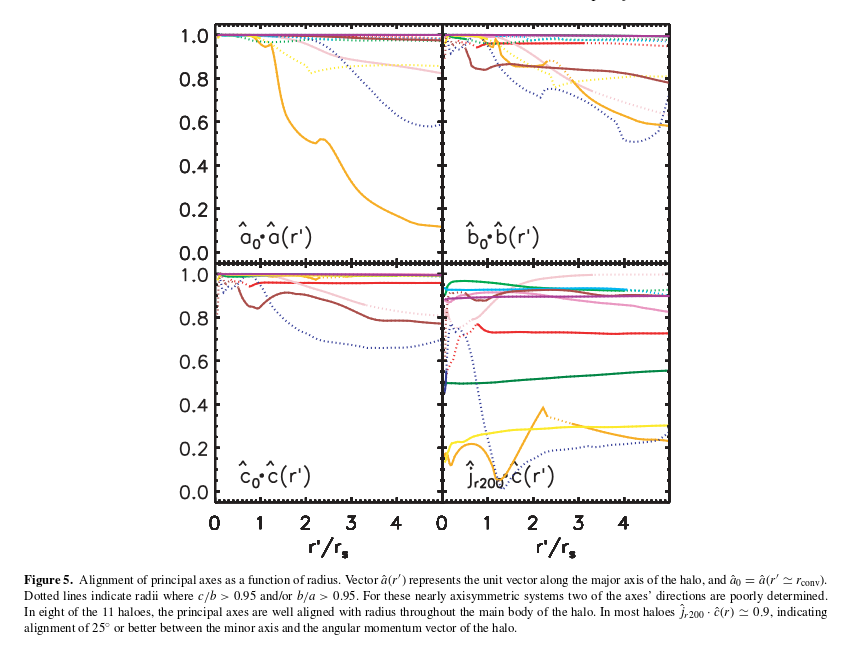
\includegraphics[scale=0.5]{alignmentH.png}
\end{figure}		

Most of the halos show a well alignment as a function of radius. 
Regarding the alignemnt of the potential with the angular momentum, they 
found that the minor axis tends to be alignment with the angular 
momentum vector 6 of 11 by $<25$. This is important because discs tend 
to be align with the halo's angular momentum. 



\section{Questions}

1. Is the MW common in LCDM
2. What is the $\hat{L}$ of the MW, is it common in LCDM?
3. Is the triaxial shape of the DM halo related with the large
scale structure in which the MW is embeded.

\end{document}

